\documentclass{../template/texnote}

\title{\textbf{How do we know the Sun's temperature?}}[author={Linn Abraham}]

\begin{document}
    \maketitle \currentdoc{note}
    %<*note>
\section{Introduction}
It is often humbling to think how far humanity has reached in its efforts to understand the cosmos.
Using the systematic knowledge building methodology that we call Science, we humans have been able to find distances to the Sun, moon and planets.
Weigh the Earth while living on just a tiny sliver of its surface called the crust.
Weigh the Sun and find the temperature and pressure in it's interior.
Most of this was done before the time of rockets and satellites with just pen, paper and the equations of science. In this article let us retrace the path that has been taken by several great thinkers and scientists who contributed to the repository of knowledge that we have today.
The primary question we want to address is how hot is the Sun? We have seen iron rods glowing red and white when heated. If so, then how much more hot must the Sun be ? What is the temperature on its surface as well as in it's core?
%\include{sections.tex}
\section{The blackbody temperature of the Sun}
A blackbody temperature or effective temperature of an object is the surface temperature that the object would have if it were a perfect blackbody.
This effective temperature can be found if one knows the luminosity of the blackbody and its surface area, using the Steffan-Boltzmann law.
The luminosity is defined as the total power radiated by the object.
A related term, apparent brightness or received energy flux, is the power per unit surface area of the detector.
This can be computed by diving the total power incident on your detector by the total surface area of your detector which would depend on your aperture size etc.
This apparent brightness is affected by the true luminosity of the object as well as the distance to the object.
For an isotropically radiating object this relationship can be expressed as,
$$ \textrm{Apparent brightness} = \frac{L}{4\pi d^2} $$
Where L is the luminosity, and d is the distance to the object.


To calculate the effective temperature for the Sun, we need to know its linear size, that is the Sun's diameter.
Since the distance to the Sun is already known, by knowing the angular size of the Sun, i.e. the angle subtended by the Sun on the sky, we can compute its linear size.
Since the Sun is very far away, the angles involved are quite small so that we can use the small-angle approximation to find this.
Doing all this we get the Sun's effective surface temperature to be 5,800 K.

\section{The Sun's core temperature}
By knowing the Sun's mass and volume we can estimate the pressure in the Sun.
By doing the calculations we find that the pressure is so high that matter can only exist in the plasma state.
That is, atoms are stripped of all its electrons.
Such a plasma is however electrically neutral on the whole and the inter-particle distances are sufficient for it to have a perfect gas behaviour.
This allows us to estimate the temperature of the plasma from the perfect gas law provided we first find out the pressure at the core.
The perfect gas law states that $ P = nkT$, where P is the pressure of the gas, n is the number density of particles and T is the temperature.
Using the law we find the temperature at the Sun's core to be $ 1.5 \times 10^7 $ K or 15 million degrees Kelvin.
%\begin{figure}[htpb]
%    \centering
%    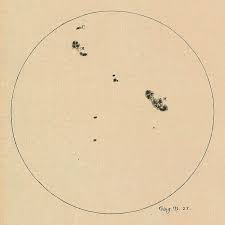
\includegraphics[width=0.48\textwidth]{Linn/sunspot_galileo_single.jpeg}
%    \caption{Original drawing of sunspots made by Galileo.} 
%    \label{fig:sunspot}
%\end{figure}


%\nocite{choudhuri_natures_2015}
%\nocite{shu_physical_1982}
%\nocite{priest_magnetohydrodynamics_nodate}
%\nocite{lemen_atmospheric_2012}

\begin{thebibliography}{4}
\providecommand{\natexlab}[1]{#1}
\providecommand{\url}[1]{\texttt{#1}}
\expandafter\ifx\csname urlstyle\endcsname\relax
  \providecommand{\doi}[1]{doi: #1}\else
  \providecommand{\doi}{doi: \begingroup \urlstyle{rm}\Url}\fi
\bibitem[1]{choudhuri_natures_2015}
Arnab~Rai Choudhuri.
\newblock \emph{Nature's Third Cycle: A Story of Sunspots}.
\newblock {Oxford University Press}, {Oxford ; New York}, 2015.
\newblock ISBN 978-0-19-967475-6.

\bibitem[2]{shu_physical_1982}
Frank~H. Shu.
\newblock \emph{The Physical Universe: An Introduction to Astronomy}.
\newblock A Series of Books in Astronomy. {Univ. Sience Books}, {Sausalito,
  Calif}, 9. print edition, 1982.
\newblock ISBN 978-0-935702-05-7.

\bibitem[3]{priest_magnetohydrodynamics_nodate}
Eric Priest.
\newblock Magnetohydrodynamics of {{The Sun}}.

\bibitem[4]{sciamerican}
\url{https://www.scientificamerican.com/article/how-do-scientists-measure/}

\bibitem[5]{cavendish}
\url{https://en.wikipedia.org/wiki/Cavendish_experiment}

\bibitem[6]{venus_transit}
\url{https://sunearthday.nasa.gov/2012/articles/ttt_75.php}

\end{thebibliography}
\vspace{0.5cm}
\noindent\fbox{%
	\parbox{\textwidth}{%
		\textbf{About the Author}\vspace{0.2cm} \\
		\textbf{Linn Abraham} is a researcher in Physics, specializing in A.I. applications to astronomy. 
He is currently involved in the development of CNN based Computer Vision tools for
prediction of solar flares from images of the Sun, morphological classifications of galaxies from optical images surveys and radio galaxy source extraction from radio observations.
	}
}
    %</note>
    \printbibliography
\end{document}
